% =====================================================
% Fig. 6 : GAA(Gate-All-Around)ナノシート構造 断面図
% =====================================================
\begin{figure}[t]
  \centering
  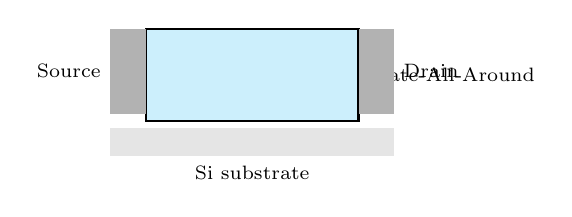
\begin{tikzpicture}[scale=0.9, every node/.style={font=\scriptsize}]
    % substrate
    \fill[gray!20] (0,0) rectangle (4,0.4);
    \node[below] at (2,0) {Si substrate};

    % nanosheets (3層)
    \foreach \y in {0.6,1.0,1.4} {
      \fill[orange!30] (0.8,\y) rectangle (3.2,\y+0.2);
      \draw[black!50] (0.8,\y) rectangle (3.2,\y+0.2);
    }

    % gate stack
    \draw[thick,fill=cyan!20] (0.5,0.5) rectangle (3.5,1.8);
    \node[right] at (3.55,1.15) {Gate-All-Around};

    % source/drain
    \fill[gray!60] (0,0.6) rectangle (0.5,1.8);
    \fill[gray!60] (3.5,0.6) rectangle (4.0,1.8);
    \node[left] at (0,1.2) {Source};
    \node[right] at (4,1.2) {Drain};
  \end{tikzpicture}

  \caption{GAAナノシート構造の模式断面図(S/D領域とゲート包囲面を示す)\\
  \footnotesize Schematic cross-section of GAA nanosheet structure showing gate wrapping around multiple stacked channels.}
  \label{fig:gaa_cross}
\end{figure}
